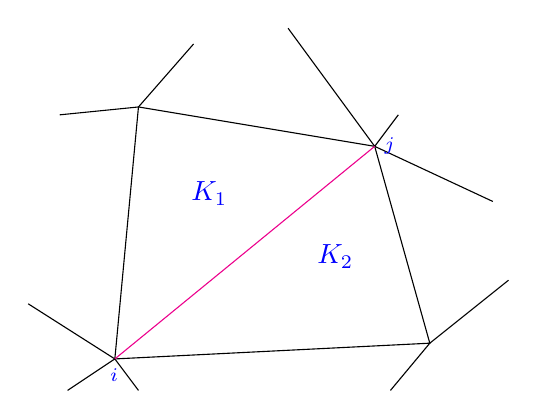
\begin{tikzpicture}
	\coordinate (A) at (0,0);
	\coordinate (B) at (4,0.2);
	\coordinate (C) at (3.3,2.7);
	\coordinate (D) at (0.3,3.2);
	
	\draw (A)--(B)--(C)--(D)--(A);	
	
	\draw (A)-- +(-.6,-.4) 		(A)-- +(.3,-.4)		(A)-- +(-1.1,.7);
	\draw (B)-- +(-.5,-.6) 		(B)-- +(1,.8);
	\draw (C)-- +(1.5,-.7) 		(C)-- +(.3,.4)	 	(C)-- +(-1.1,1.5);
	\draw (D)-- +(-1,-0.1) 		(D)-- +(.7,.8);
	
	\draw[magenta] (A)--(C);
	
	\node[text=blue] at (1.2,2.1) {$K_1$};
	\node[text=blue] at (2.8,1.3) {$K_2$};
	\node[text=blue,anchor=north] at (A) {$\bx_i$};
	\node[text=blue,anchor=west] at (C) {$\bx_j$};	
\end{tikzpicture}
